% Figure M1, generated by experiments/m1_multilayer.py.
\begin{figure}[t]
  \centering
  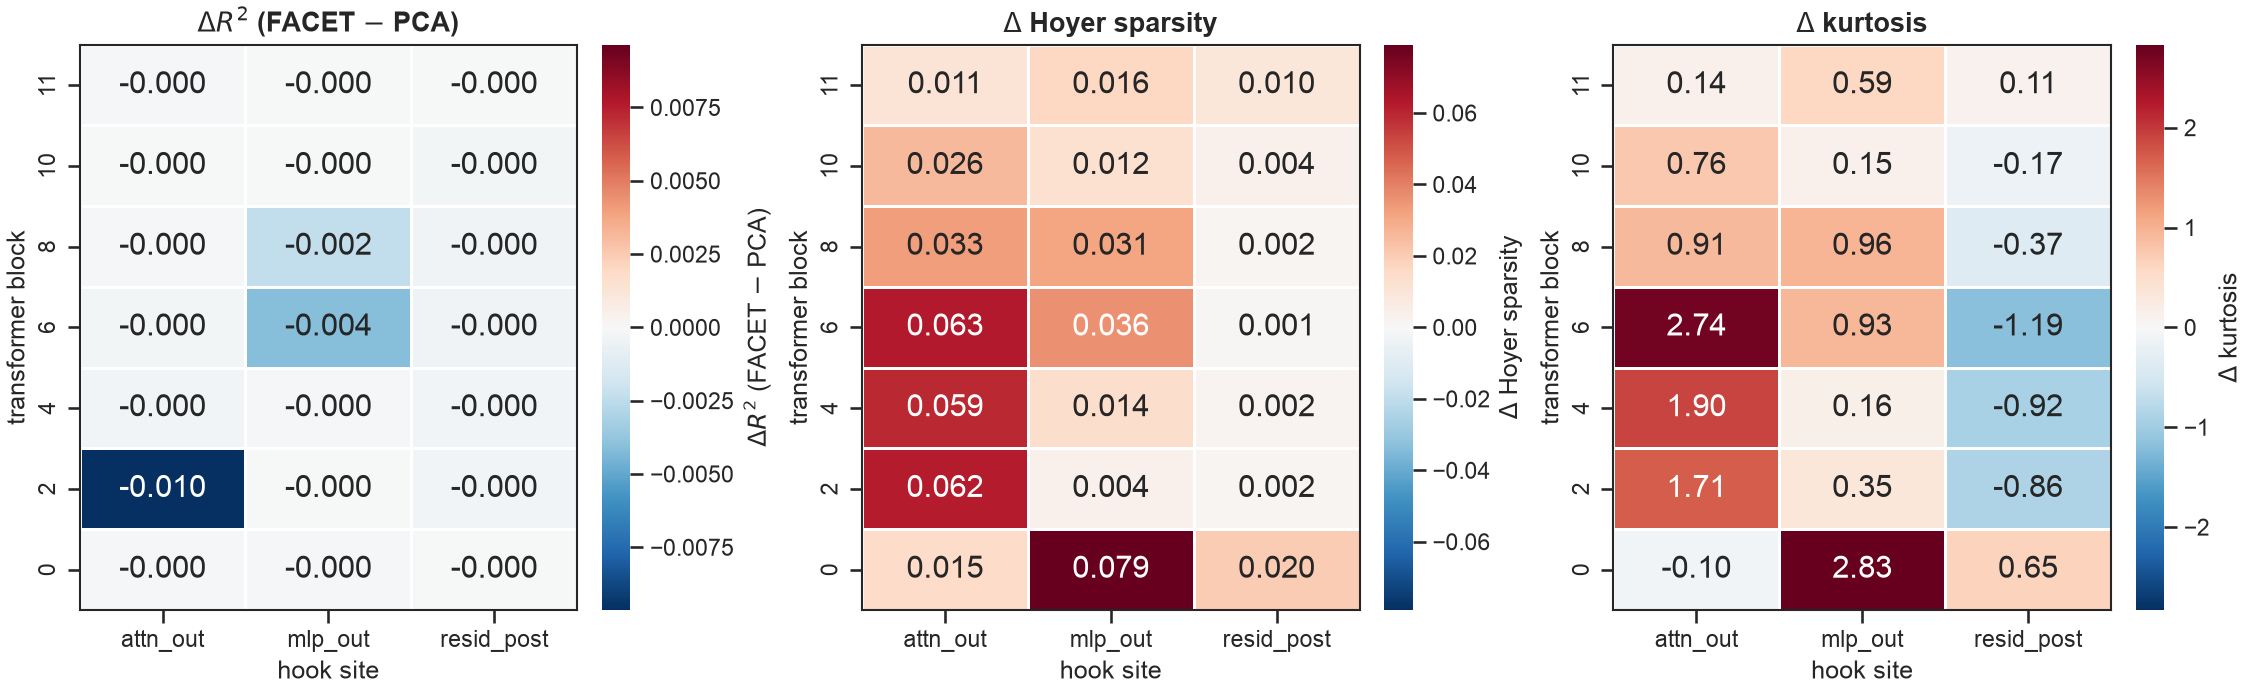
\includegraphics[width=\linewidth]{../shared/figures/generated/m1_multilayer.png}
  \caption{\textbf{M1, FACET $-$ PCA gap across GPT-2 small layers and hook sites.} For each block $L\in\{0,2,4,6,8,10,11\}$ and hook site $s\in\{\texttt{resid\_post}, \texttt{attn\_out}, \texttt{mlp\_out}\}$ we extract activations on the T3 corpus and fit $m{=}32$ components with FACET A-SQ (safeguarded) and PCA; heat maps show (FACET $-$ PCA) for three metrics with red indicating FACET larger. \textit{Left:} reconstruction $R^2$ is within $[-0.01, 0]$ of PCA on every cell, FACET pays no representational cost. \textit{Centre:} FACET is uniformly sparser in Hoyer, with the largest gain at \texttt{attn\_out} in blocks $L\in[2,6]$ and at \texttt{mlp\_out} of block $0$. \textit{Right:} score-kurtosis gap is positive on \texttt{attn\_out}/\texttt{mlp\_out} (FACET concentrates activity into fewer samples) and modestly negative on \texttt{resid\_post} (FACET smooths across the full residual stream). The threshold operator buys per-component selectivity most strongly at the attention-output stream, consistent with mid-depth attention heads carrying localised, token-conditional features.}
  \label{fig:m1-multilayer}
\end{figure}
